\chapter{VR Interface}

In this chapter, I'll go into the implementation details of the VR interface. 
The requirements for the interface are as follows:
\begin{enumerate}
    \item It needs to report the 6-DOF poses of left and right hands as well as additional buttons for locomotion and gripper control. 
    \item Stereoscopic images need to be streamed and displayed on the VR headset to create depth perception for the wearer. 
    \item It needs to connect to both the simulation codebase written in Python and the real-robot controller written in C++. 
    \item The latency should be low and the computation speed should be fast so that the wearer can provide demonstrations with ease. The computation resource consumption should be low because the simulation and whole-body controller are resource-intensive.
\end{enumerate}

First, an overview of the architecture is given. Then, I justify some of the design decisions. Finally, I analyze the performance of the system.

\section{Architecture}

\begin{figure}
	\centering
	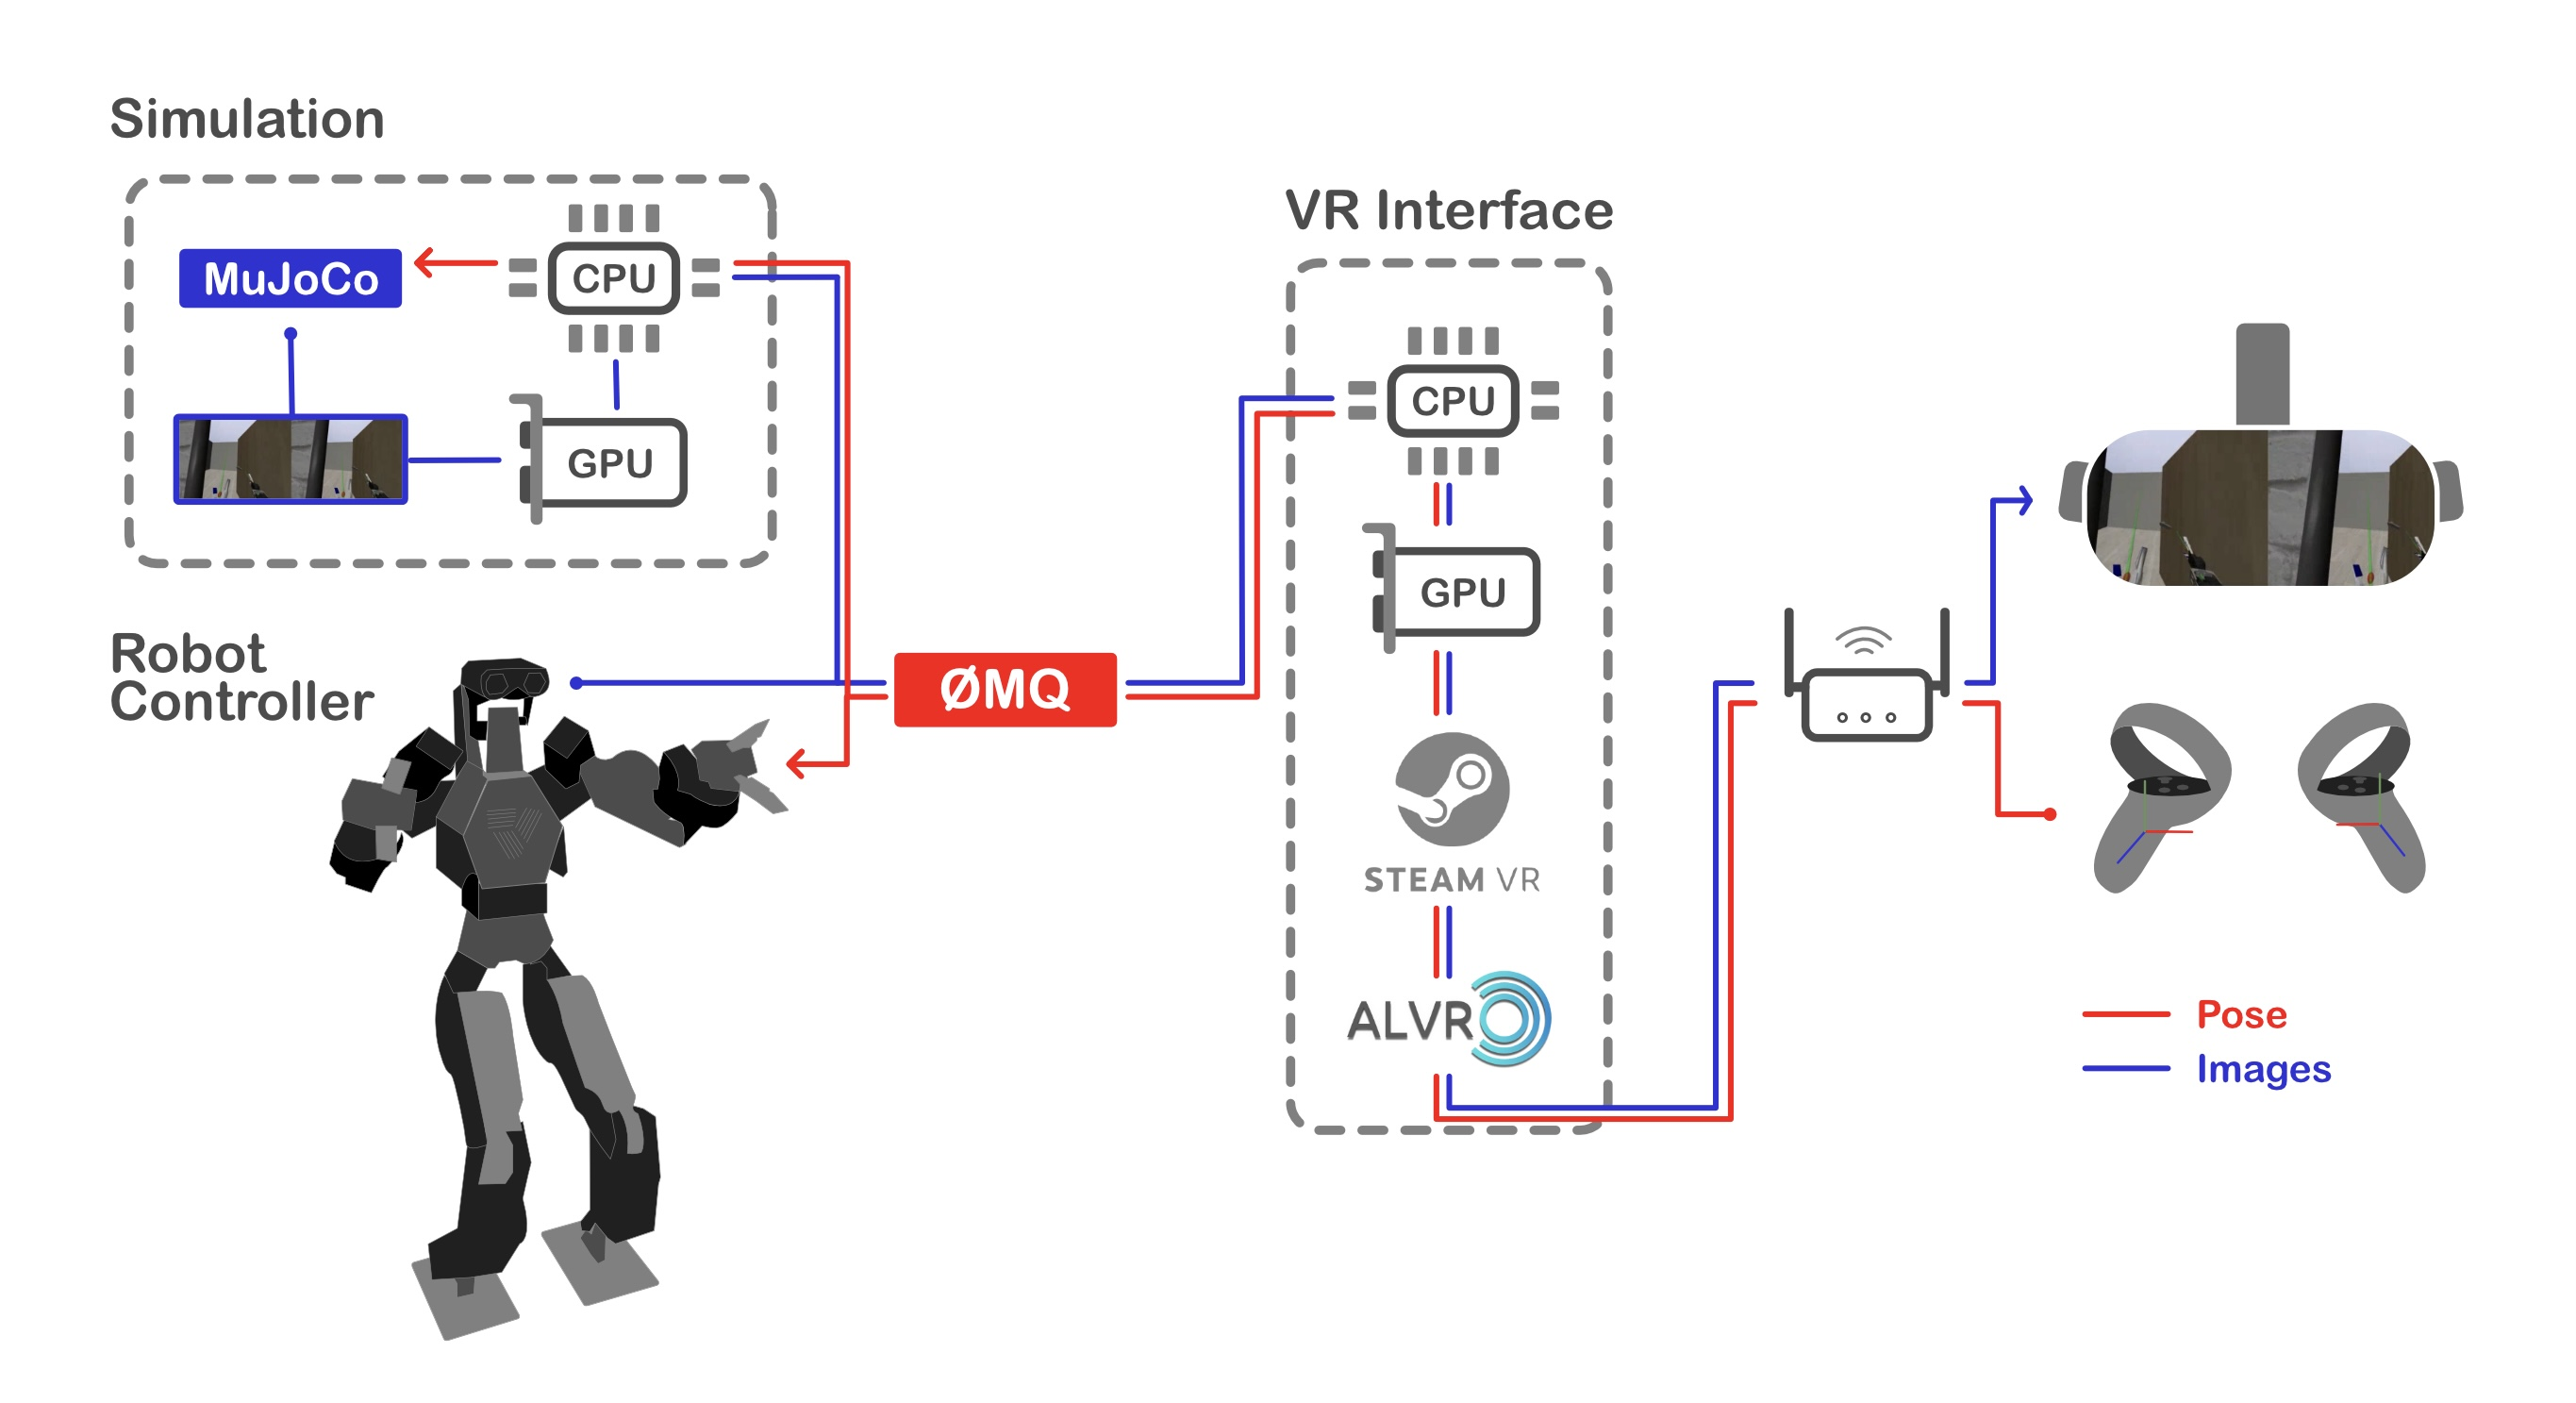
\includegraphics[width=\linewidth]{architecture_diagram.jpeg}
	\caption{Architecture for the VR interface}
    \label{fig:vr-interface}
\end{figure}

Figure \ref{fig:vr-interface} describes the software architecture. The VR interface code written in C++ runs on a separate laptop, which is connected to either the simulation desktop or the robot control station for the real robot. We use OpenVR (implemented in SteamVR) and ALVR (Air Light VR) for the communication between the laptop and the headset. OpenVR is a low-level API for VR applications designed to support a wide range of VR devices. ALVR is an open-source project that allows streaming Steam VR games from the laptop to the headset via Wi-Fi. It implements technologies such as Asynchronous Timewarp and Fixed Foveated Rendering for a smoother experience. ZMQ is an asynchronous messaging library that simplies message-passing between different programs or devices. 

For the simulation, we use Mujoco with Python binding for the physical simulation and Robosuite for the objects in the scene. We first render the scene using a virtual stereoscopic camera that is adjusted to match the interpupillary distance of the VR headset. Then, the rendered pixels are copied from the GPU to CPU and sent to the VR interface using ZMQ and ethernet. The interface code listens to the images and writes them into a GPU texture used by OpenVR. Finally, SteamVR and ALVR transmits the images through a router and displays them in the VR headset. At the same time, the interface polls the VR headset for the poses of the headset and controllers through OpenVR. It transforms the controller poses to the local frame of the headset, and they are then mapped to the poses of the robot hands in the robot's local frame. The latter mapping involves aligning the rotation axes of the controller with the axes used in the simulation. Let $R_t$ be the transformation between the VR axes and the simulation axes, $R_{vr}$ be rotation of the controller from its natural orientation, and $R_{sim}$ be the desired rotation to be applied to the robot hands. Their relation can be expressed as 
$$
R_{sim} = R_t^{-1} R_{vr} R_t
$$
The transformed hand poses are then published continuously using a ZMQ pub socket. When the simulation needs a VR command, it pulls the most recent command from the queue and sends it to the whole-body controller. 

The setup for the real robot is similar. However, since the robot has a lot more components to manage, it will be described in more details in the next chapter.

\section{Design Choices}

Some difficult design decisions were made to satisfy the requirements defined above. They are explained in the section in hopes of providing documentation and guidance for others working on similar systems.

\subsection{OpenVR}

Initially, a website was created based on WebXR and JavaScript to stream controller poses over the internet. I wanted to improve the latency by keeping the connection within a local network, but I encountered difficulty in setting up HTTPS certificates in the campus lab. After getting tired of tunneling the connection over the internet, I decided to pursue a more low-level approach. 
The native Oculus SDK could work, but it would limit the option to change VR systems in the future. Unity is a good option for cross-platform compatibility, but since there's only a need to stream images and controller poses, a game engine is an overkill. I also don't believe that Unity exposes the low-level functionality to directly show the stereoscopic images. Since Unity uses the low-level OpenVR API, I decided to use it directly. Although a newer API called OpenXR is gaining steam, I feel that the performance benefits of OpenXR doesn't justify its complexity compared to OpenVR. 

Using OpenVR has several advantages. First, it has great performance since it is used by VR games and has direct support from VR headset manufacturers. The fact that all SteamVR games use it also makes it suitable for my proposal to embed the demonstration collection system in video games. Second, it delegates the work of video streaming to existing technologies. Many VR headsets support direct HDMI connection from the computer's graphics card, which OpenVR can take full advantage of since it takes input images from OpenGL. Even though the Quest doesn't have an HDMI cable, it is still possible to use the Oculus Link (over an USB cable) or Oculus Air Link (over a local network) with OpenVR. These are sophisticated streaming technologies that predict the user's movements and streaming latency to render ahead of time, and they encode the frames as slices in H.264 \cite{air-link}. ALVR is an open-source alternative that implements similar technologies with the added benefit of having experimental support for Linux. This is much more performant and scalable than hand-coding an image streaming pipeline, as done by \cite{arunachalam2022holodex}. Finally, OpenVR works on a variety of Operating Systems and targets many VR headsets. My code readily runs on Windows laptops just like Linux.

\subsection{Image Transfer from GPU to CPU}

Since our interface script is written in C++ (since the Python OpenVR binding doesn't work well) while the simulation is in Python, we need a way to transfer the rendered images between processes. 
First, we can use memory sharing or pybind to transfer the Mujoco simulation state. Using the simulation states, the C++ code can directly render the scene using Mujoco and pass the result directly to OpenVR within the GPU. However, since Mujoco allocates simulation data structure dynamically, it's difficult to do inter-process memory sharing. Second, we could hypothetically share the GPU buffer rendered by the python script with the C++ script, but OpenGL contexts don't seem to allow inter-process sharing. Third, we can lose some performance and transfer the images from GPU to CPU. Once the images are in memory, we can send them over using ZMQ. 

The last approach was chosen to make the design more adaptable to the real robot, where the images are always coming from memory. The rendered images have a resolution of $1096 \times 2$ by $1176$, where the width is multiplied by 2 to account for both eyes. The rendering of an image takes .3 milliseconds on the RTX3090 GPU, copying it to the CPU consumes 3 milliseconds, and sending it through ZMQ uses .6 milliseconds. Overall, this number is negligible compared to the simulation and whole-body control times, so this performance is acceptable. 

\subsection{Asynchronous Message Passing}

The simulation uses a ZMQ sub socket to get actions from the pub socket in the interface script. Usually this is done synchronously, meaning that the simulation waits for the interface to provide a response after requesting. However, this approach usually takes 70 milliseconds for the message round-trip. This delay can be reduced to .1 milliseconds by using an asynchronous approach. In this case, the sender and receiver simply run at their own pace, and the ZMQ threads in the background takes care of getting the messages ready. When the simulation requests an action, the ZMQ simply gets the most recently received message in its queue and returns it. Since the interface runs at a higher frequency than the simulation, there will never be a case where no action is available. Also, by setting the "conflate" option in ZMQ, we can reduce the need of a queue by only keeping the most recent message. 

\subsection{Separate Computer for VR Interface}

At first, the simulation and interface scripts ran on the same desktop computer. However, we noticed that the scripts were competing for resources, causing performance degradation. We chose ALVR since it's the only option on Linux to connect to VR, and its wireless design enables remote teleoperation. However, encoding the stream in real time consumes CPU power needed for the whole-body controller. When running, the simulation and whole-body controller takes up 1500\% of the CPU, while ALVR and SteamVR consume around 200\%. After decoupling the VR interface to a separate laptop, we noticed around 10\% performance improvement.

\section{Performance Analysis}
The performance of the VR Interface is acceptable. Using asynchronous message passing and a separate laptop for VR interface, receiving images and sending commands are both sub-millisecond operations. The biggest contributor to latency is ALVR, which adds about 70 milliseconds of latency. However, this is nothing compared to the latency introduced by slow simulation. In the simulation loop, for every rendering and communication with the interface, we run 25 simulation steps and 5 whole-body control computations. In comparison, on the hardware, the whole-body control code is run 20 times between every two action inputs. This means that in simulation, the whole-body control code may not have reached the desired action before a new action is given. Indeed, the slow tracking speed of the whole-body control introduces a large delay between the movement of the controller and the robot's hands reaching the desired poses. We qualitatively assessed this by rendering the desired poses as arrows in simulation, and we found that for fast motions, the robot can take up to a second to reach the desired state. 
\begin{figure}
	\centering
	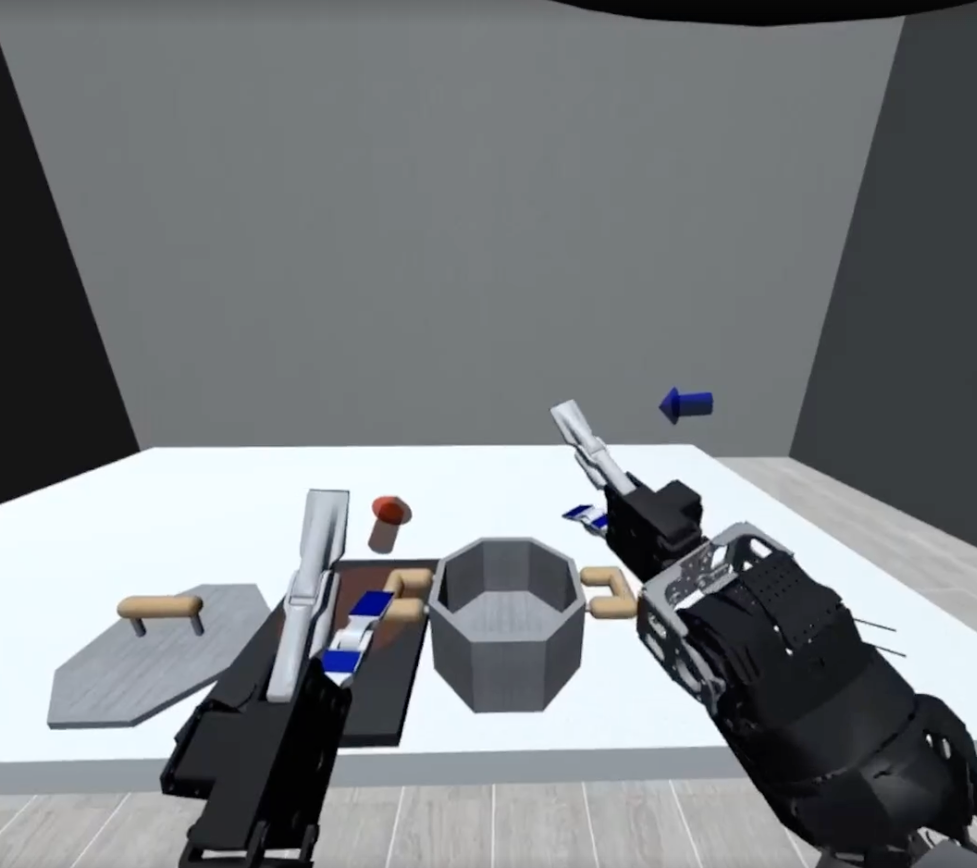
\includegraphics[width=15em]{arrows.png}
	\caption{The robot hands takes time to reach the desired controller poses (represented by arrows).}
    \label{fig:arrows}
\end{figure}

Another big issue with the current setup is speed. The current simulation loop can only achieve around 10 fps in the contact-rich kitchen environment. This is also the reason we can't simply increase whole-body control computation frequency. A humanoid robot capable of walking requires an accurate physical simulation. We are using Mujoco with the RK4 integrator and PGS numerical solver at 50 iterations per time step, where the time step is set at 2 milliseconds. We have also tried running the numerical solver at 10 iterations per time step, sacrificing some precision for speed. For debugging, we also tried rendering the images using OpenCV instead of sending them to the VR headset. Some performance numbers are shown in Table \ref{table:perf}. Since the quickest loop time is 70 milliseconds, there is no hope that our setup can reach 60 fps. From the table, we see that using OpenCV to display images takes quite a lot of time, whereas sending the images to VR is faster. When walking is not involved, the whole-body controller time is reduced drastically, while manipulation tasks involving contact slows down Mujoco. Overall, Mujoco and whole-body control are the biggest culprits for performance issues. 

\begin{table}[h]
\scriptsize
\begin{center}
\caption{Simulation performance numbers. The left column denotes whether OpenCV or the VR headset is used to display the image and the number of PGS iterations per time step. The last row shows a manipulation task without locomotion. In each loop, Mujoco runs 25 times, WBC runs 5 times, and rendering runs once. The first three columns measure the time taken in each run, the fourth column shows the total time taken by each loop, while the last three columns show their percent contribution to total loop time considering the number of times they run.  }
\vskip 10pt
\begin{tabular}{|c|c|c|c|c|c|c|c|}
\hline
& Mujoco (ms) & Render (ms) & WBC (ms) & Total (ms) & Mujoco & Render & WBC\\
\hline
	CV, 50 & 1.72 & 30 & 7.7 & 120 & 35\% & 27\% & 31\% \\
\hline
	CV, 10 & .8 & 30 & 7.7 & 100 & 21\% & 33\% & 39 \% \\
\hline
	VR, 50 & 1.72 & 8 & 6 & 92 & 48\% & 8\% & 34\% \\
\hline 
	VR, 10 & .92 & 8 & 6 & 70 & 33\% & 11\% & 44\% \\
\hline 
	
	\begin{tabular}[x]{@{}c@{}}VR, 50\\no walking\end{tabular}& 2.12 & 8 & 5 & 90 & 57\% & 8\% & 25\%\\
	\hline
\end{tabular} \\[10pt]
\vskip -20pt
\end{center}
\label{table:perf}
\end{table}


However, this is not the end of the story for potentially embedding our setup in a video game. As mentioned, our simulation codebase is written in Python. When the C++ codebase from the hardware team is used, each WBC computation is reduced from 5 to .45 milliseconds. In fact, the hardware team has their own simple simulation in PyBullet for debugging purposes. As mentioned before, they run 20 simulation steps and 20 WBC calls per loop. On the same machine, their loop is able to execute 40 times per second with the VR interface. Needless to say, one of our current tasks is to substitute our Python code with their C++ code.
